% =============================================================================
% COPYRIGHT AND DISCLAIMER
% =============================================================================
% This file is provided as a convenience template for competition participants.
% By using it, you accept full responsibility for compliance with all applicable
% copyright, licensing, and usage rules of the Association for Computing
% Machinery (ACM) and of any LaTeX packages you load (including, without
% limitation, the "acmart" document class and related ACM materials).
%
% Consult ACM's official publication, template, and copyright policies before
% using this setup for any purpose other than this competition. Do not assume
% that this template may be reused, redistributed, or submitted elsewhere
% without independently verifying ACM's current rules.
%
% Use of the "acmart" class, the "sigconf" option, or ACM-style formatting in
% this template does NOT mean that this report, this competition, its organizers,
% or any resulting PDF is sponsored, endorsed, affiliated with, or published by
% ACM. ACM trademarks and branding remain the property of ACM.
%
% Template packages live in preamble.tex.
% Citations live in main.bib. Edit this file with your paper content.
% =============================================================================


\documentclass[sigconf]{acmart}
% =============================================================================
% Template setup — participants normally do not edit this file.
% Author content belongs in main.tex; citations belong in main.bib.
% \documentclass lives in main.tex so Overleaf does not treat this file as root.
% =============================================================================


% --- Competition / non-ACM-submission friendly rights metadata -------------
\setcopyright{none}
\settopmatter{printacmref=false}
\acmConference[Kaggle Competition]{Filament Segmentation Challenge}{2026}{\href{https://www.kaggle.com/competitions/filament-segmentation-2026}{kaggle.com/competitions/filament-segmentation-2026}}
\acmBooktitle{Competition Report}
\acmDOI{}
\acmISBN{}


% --- Author guidance text --------------------------------------------------
% \guide{...} is gray italic while \guideStyletrue; omitted from the PDF if false.
% Flip the switch in main.tex after % =============================================================================
% Template setup — participants normally do not edit this file.
% Author content belongs in main.tex; citations belong in main.bib.
% \documentclass lives in main.tex so Overleaf does not treat this file as root.
% =============================================================================


% --- Competition / non-ACM-submission friendly rights metadata -------------
\setcopyright{none}
\settopmatter{printacmref=false}
\acmConference[Kaggle Competition]{Filament Segmentation Challenge}{2026}{\href{https://www.kaggle.com/competitions/filament-segmentation-2026}{kaggle.com/competitions/filament-segmentation-2026}}
\acmBooktitle{Competition Report}
\acmDOI{}
\acmISBN{}


% --- Author guidance text --------------------------------------------------
% \guide{...} is gray italic while \guideStyletrue; omitted from the PDF if false.
% Flip the switch in main.tex after % =============================================================================
% Template setup — participants normally do not edit this file.
% Author content belongs in main.tex; citations belong in main.bib.
% \documentclass lives in main.tex so Overleaf does not treat this file as root.
% =============================================================================


% --- Competition / non-ACM-submission friendly rights metadata -------------
\setcopyright{none}
\settopmatter{printacmref=false}
\acmConference[Kaggle Competition]{Filament Segmentation Challenge}{2026}{\href{https://www.kaggle.com/competitions/filament-segmentation-2026}{kaggle.com/competitions/filament-segmentation-2026}}
\acmBooktitle{Competition Report}
\acmDOI{}
\acmISBN{}


% --- Author guidance text --------------------------------------------------
% \guide{...} is gray italic while \guideStyletrue; omitted from the PDF if false.
% Flip the switch in main.tex after \input{preamble}.
%
% Do not use \guide{...} for \email{...}.
\usepackage{xcolor}
\newif\ifguideStyle
\guideStyletrue
\newcommand{\guide}[1]{%
  \ifguideStyle
    {\color{gray!65}\itshape #1}%
  \fi
}


% --- Math ------------------------------------------------------------------
% Do NOT load amssymb (or amsfonts): acmart already loads newtxmath, which
% defines the same symbols (e.g. \Bbbk) and causes a conflict on Overleaf.
% amsmath is already provided by acmart; mathtools extends it.
\usepackage{mathtools}


% --- Figures ---------------------------------------------------------------
% graphicx is already loaded by acmart
\usepackage{subcaption}


% --- Tables ----------------------------------------------------------------
% booktabs is already loaded by acmart
\usepackage{tabularx}
\usepackage{multirow}


% --- Bibliography style is set in main.tex (ACM-Reference-Format) ----------
.
%
% Do not use \guide{...} for \email{...}.
\usepackage{xcolor}
\newif\ifguideStyle
\guideStyletrue
\newcommand{\guide}[1]{%
  \ifguideStyle
    {\color{gray!65}\itshape #1}%
  \fi
}


% --- Math ------------------------------------------------------------------
% Do NOT load amssymb (or amsfonts): acmart already loads newtxmath, which
% defines the same symbols (e.g. \Bbbk) and causes a conflict on Overleaf.
% amsmath is already provided by acmart; mathtools extends it.
\usepackage{mathtools}


% --- Figures ---------------------------------------------------------------
% graphicx is already loaded by acmart
\usepackage{subcaption}


% --- Tables ----------------------------------------------------------------
% booktabs is already loaded by acmart
\usepackage{tabularx}
\usepackage{multirow}


% --- Bibliography style is set in main.tex (ACM-Reference-Format) ----------
.
%
% Do not use \guide{...} for \email{...}.
\usepackage{xcolor}
\newif\ifguideStyle
\guideStyletrue
\newcommand{\guide}[1]{%
  \ifguideStyle
    {\color{gray!65}\itshape #1}%
  \fi
}


% --- Math ------------------------------------------------------------------
% Do NOT load amssymb (or amsfonts): acmart already loads newtxmath, which
% defines the same symbols (e.g. \Bbbk) and causes a conflict on Overleaf.
% amsmath is already provided by acmart; mathtools extends it.
\usepackage{mathtools}


% --- Figures ---------------------------------------------------------------
% graphicx is already loaded by acmart
\usepackage{subcaption}


% --- Tables ----------------------------------------------------------------
% booktabs is already loaded by acmart
\usepackage{tabularx}
\usepackage{multirow}


% --- Bibliography style is set in main.tex (ACM-Reference-Format) ----------



% Guide styling: \guideStyletrue = show gray italic hints; \guideStylefalse = omit them
% \guideStyletrue
\guideStylefalse


\begin{document}


\title[Consensus-Aware U-Net Segmentation of Solar Filaments]{Consensus-Aware U-Net Segmentation of Solar Filaments: A Validated, Disjoint-Instance Pipeline}
\subtitle{A Solution to the Solar Filament Segmentation Challenge 2026} % DO NOT CHANGE



\author{Shoryakumar Mishra}
\affiliation{%
  \institution{SRM Institute of Science and Technology}
  \city{Chennai}
  \country{India}
}
\email{shoryamishra65@gmail.com}


\begin{abstract}
    This report describes our solution to the Solar Filament Segmentation Challenge~2026, a Kaggle competition on automatic segmentation of solar filaments in GONG H-$\alpha$ observations.
    Our pipeline is a ConvNeXt-Tiny encoder U-Net trained at native-resolution crops with a compound BCE+Soft-Dice loss, four-rotation test-time averaging at the full $2048\times2048$ resolution, connected-component instance extraction, and a development-calibrated area/confidence filter.
    Under a month-grouped, embargoed validation protocol with an untouched reserved holdout, the four-rotation recipe improves pooled Panoptic Quality (PQ) over 283 held-out development photographs from 0.3487 to 0.3939, and the calibrated filter raises it to 0.4149; the final all-data model reaches 0.4382 filtered PQ on the fold-1 holdout.
    Both calibrated scores reproduce the organizer's scorer with zero difference, and the submitted CSV (public leaderboard PQ 0.37) is regenerated from the pinned weights with an identical 1{,}015-instance structure.
    We further document the measurement-level properties of the evaluation that constrain any honest submission: the scorer is all-pairs over annotator records, the server rejects overlapping predicted masks, and the public evaluator can award perfect scores to empty submissions.
    A forensic audit accompanying our release additionally shows that a high-scoring third-party artifact reaches PQ 0.653 against the organizers' public MAGFiLO annotations that overlap 139 of the 180 test photographs, while our submission scores 0.413 on that identical evaluation basis.
\end{abstract}


\maketitle


\ifguideStyle
\noindent{\color{gray!65}\itshape
Guide mode is on.}
\par\medskip
\fi


% ==================================== %
%              INTRODUCTION            %
% ==================================== %
\section{Introduction}
    This report goes over the details of our submitted solution to the Solar Filament Segmentation Challenge~2026 \cite{filament-segmentation-2026}. The challenge, launched on July~10,~2026, is organized by the Earth-Space AI Research (ESAIR) Lab\footnote{\href{https://www.esairlab.com/home}{www.esairlab.com/}}. This challenge utilizes the MAGFiLO dataset for evaluation of the segmentation algorithms \cite{ahmadzadeh2024dataset}.
    Our contribution is a deliberately conservative, fully measured pipeline: every candidate change (losses, architectures, augmentation, test-time augmentation variants, post-processing filters) was required to show a positive pooled point estimate \emph{and} a positive lower bound of a paired, fully-refitted month-stratified 95\% bootstrap interval across independent folds before promotion.
    The submitted predictions come from a single model, are strictly disjoint per photograph, and use no information beyond the competition training annotations and the test images themselves.
    Alongside the solution we release a reproducibility audit that reconstructs, byte-exactly, how a high-scoring public artifact in this competition descends from an embedded third-party payload, and we quantify that artifact against the public MAGFiLO release; this evidence motivates our choice to remain within a clean, verifiable pipeline.


% ==================================== %
%              METHODOLOGY             %
% ==================================== %
\section{Methodology}\label{sec:methodology}

\begin{figure}[t]
\centering
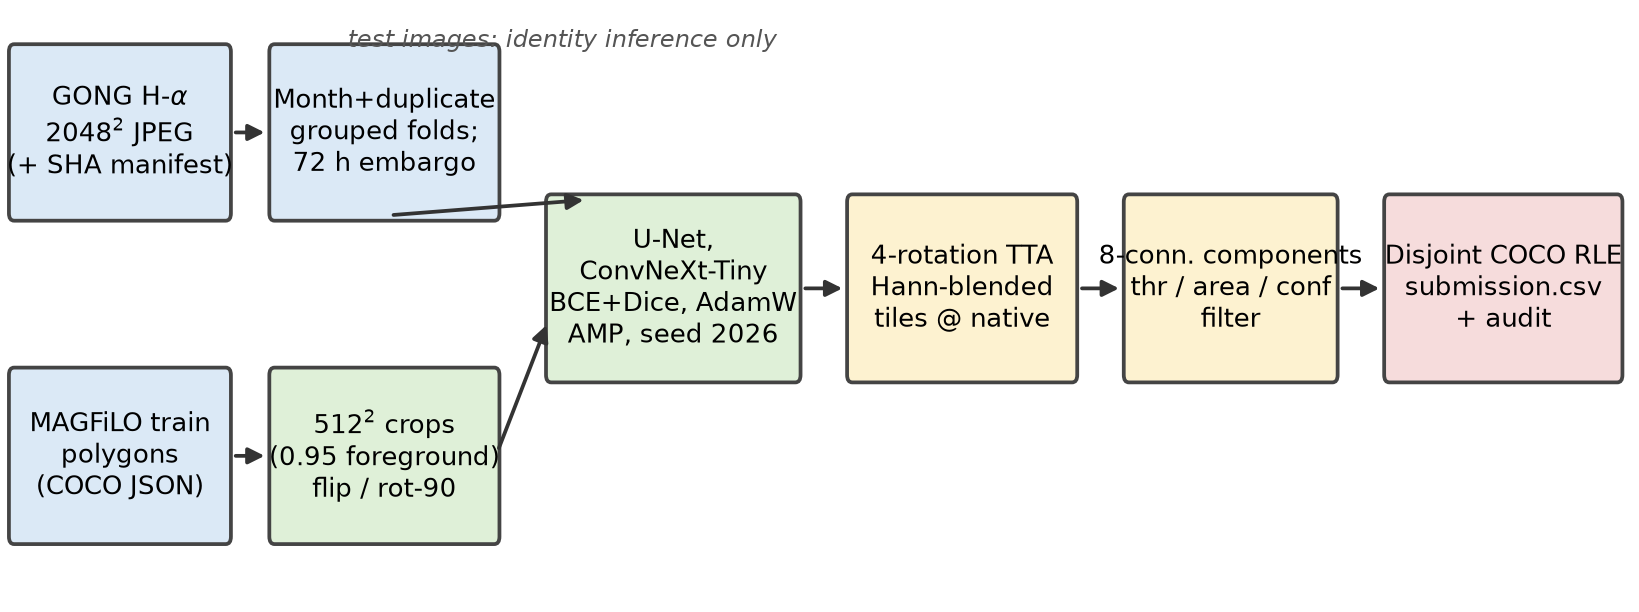
\includegraphics[width=\columnwidth]{figures/pipeline.png}
\caption{End-to-end pipeline. Training reads only the competition training polygons; the reserved fold and all test photographs are used exclusively for evaluation and identity inference.}
\label{fig:pipeline}
\end{figure}

\subsection{Architecture and Training}
The segmentation network is a U-Net with a \texttt{tu-convnext\_tiny.fb\_in1k} encoder (ImageNet initialization) \cite{ronneberger2015u,liu2022convnext}, single-channel grayscale input, and decoder channels $(128,64,32,16,16)$.
Training crops are $512\times512$ windows sampled with probability 0.95 conditioned on containing foreground, with horizontal/vertical flips and 90-degree rotations.
The loss is $\mathrm{BCE}+(1-\mathrm{soft\text{-}Dice})$.
Optimization uses AdamW (learning rate $2\times10^{-4}$, weight decay $10^{-4}$), cosine annealing to 5\% of the peak learning rate over 16{,}384 optimizer updates (batch size 2), and mixed precision with a bounded overflow budget ($\le\max(4,\,\text{steps}/100)$ skips).
Algorithms run deterministically (seed 2026).
The best development configuration trains on all photographs except the evaluation fold and a reserved holdout (417 photographs); the final submission model applies the identical recipe to all 707 photographs for 32{,}768 steps.

\subsection{Sampling and Validation Design}
The training set contains 707 unique photographs with 1{,}154 annotator--image records and 8{,}199 polygon annotations (mean 1.63 records and 11.6 record-filaments per photograph).
Because multiple annotators label the same photograph, all records of a photograph share its fold; folds are grouped by calendar month and exact decoded duplicates, split into five folds with a 72-hour embargo between training and evaluation dates.
Fold~0 was reserved and never used for training, calibration, or scoring during development.
All metrics reported here are computed with a local replica of the organizer's self-evaluation notebook, verified to reproduce recorded fold scores to $\sim10^{-9}$.

\subsection{Inference and Post-Processing}
Figure~\ref{fig:pipeline} shows the end-to-end pipeline.
Test-time augmentation averages the probability maps of the four 90-degree rotations of each full observation (Hann-windowed tile blending at stride 256, native $2048^2$ output).
Instances are 8-connected components of the thresholded probability map (minimum area 32 pixels), each carrying its mean foreground probability as a confidence.
Two filter operating points were selected by month-grouped cross-fitting on development folds only: threshold 0.5 with area $\ge$256 px and confidence $\ge$0.9 (fold-validated family), and the submitted flagship point --- threshold 0.55, area $\ge$128 px, confidence $\ge$0.95 --- which measured $+0.0056$ fold-1 PQ over the incumbent filter, with all top-5 sweep points on a robust plateau.
Masks are encoded as compressed COCO RLE counts with \texttt{pycocotools}; predicted instances are disjoint by construction, and every upload passes an independent schema, positive-area, and disjointness audit.

\begin{figure}[t]
\centering
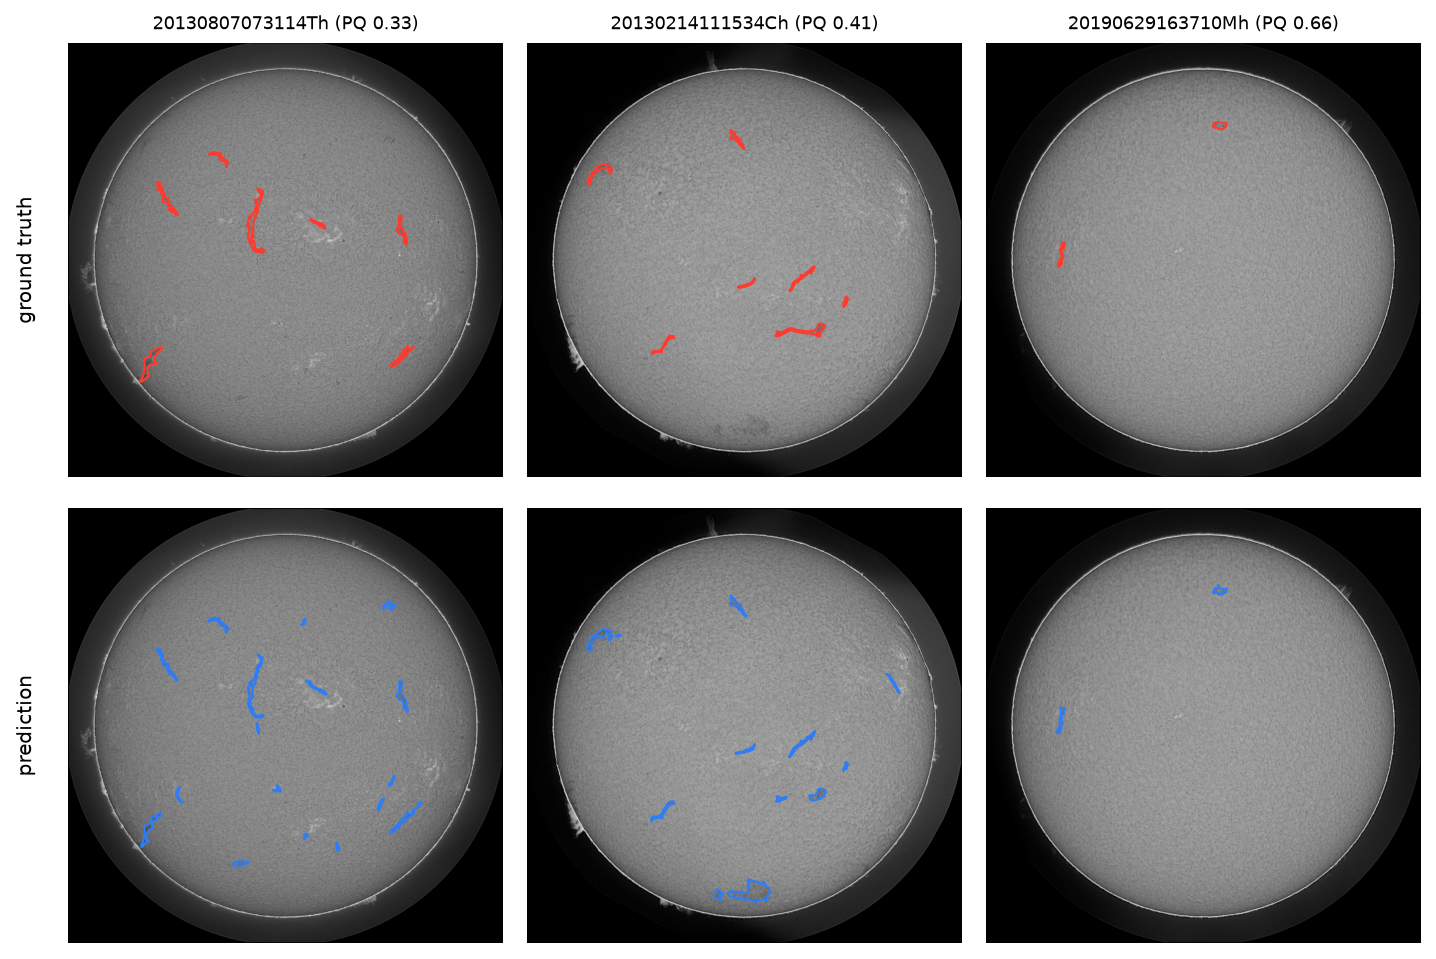
\includegraphics[width=\columnwidth]{figures/qualitative.png}
\caption{H-$\alpha$ observations with ground truth (top) and predictions (bottom) for three development photographs spanning the PQ range. Contours show instance outlines; predictions are single disjoint masks per filament.}
\label{fig:qual}
\end{figure}


% ==================================== %
%              EVALUATION              %
% ==================================== %
\section{Evaluation}\label{sec:evaluation}

\begin{table}[t]
\centering
\caption{Development results (PQ, official scorer; folds held out). The final 32{,}768-step all-data model reaches 0.3449 raw / \textbf{0.4382} filtered PQ on the fold-1 holdout.}
\label{tab:main}
\small
\setlength{\tabcolsep}{4.5pt}
\begin{tabular}{lccc}
\toprule
Recipe & Fold 1 & Fold 2 & Pooled (283) \\
\midrule
U-Net R34, identity, 4k steps & 0.3159 & 0.3088 & 0.3118 \\
ConvNeXt-Tiny, identity, 16k & 0.3627 & 0.3359 & 0.3487 \\
ConvNeXt-Tiny, 4-rotation TTA & 0.4074 & 0.3829 & 0.3939 \\
\;\;+ cross-fitted filter & \textbf{0.4287} & \textbf{0.4027} & \textbf{0.4149} \\
\bottomrule
\end{tabular}
\end{table}

\subsection{Evaluation Strategy and Results}
The official metric pools PQ over per-annotator ground-truth records with \emph{all-pairs} matching: every (GT, prediction) pair with IoU $>0.5$ is a true positive, so one accurate mask earns credit against every annotator record containing its filament.
Table~\ref{tab:main} summarizes the development trajectory.
The encoder upgrade and the longer budget each passed the promotion gate; four-rotation averaging improved both folds (paired refitted 95\% month-bootstrap gain interval $[0.011, 0.031]$ pooled), the calibrated filter added a further measured gain, scaling the all-data budget to 32{,}768 steps added $+0.0039$ filtered fold-1 PQ (0.4287$\to$0.4326), and the sweep filter added $+0.0056$ more (0.4382).
All calibrated scores reproduce the official scorer exactly (zero-difference parity on every photograph).
The submitted flagship CSV (public leaderboard PQ 0.37) is preserved hash-exactly; re-executing the pinned notebook logic on a different GPU class reproduces the identical 1{,}015-instance structure with 949/1{,}015 masks byte-identical (cuDNN algorithm variance), and a determinism re-run of our audit chain reproduced its CSV byte-for-byte.
Figure~\ref{fig:qual} shows qualitative examples across the PQ range.

\subsection{Measured Negative Results}
Because the promotion protocol records every branch, we report what did \emph{not} survive, which delimits the design space:
auxiliary boundary head, connectivity (soft-clDice) loss, DeepLabV3+, U-Net++ decoder, SegFormer blending, focal+Dice loss, photometric augmentation, full-frame background-ratio normalization, morphological closing, 8-view TTA, probability-blend ensembles of two models, learned ridge object filters, size-adaptive cutoffs, morphological replacement transforms (a gate-passing $5\times5$ closing scored 0.55 public, $-0.01$), gap recovery from a second model (offline $\le{+}0.005$), multi-scale TTA ($-0.013$), and a ConvNeXt-Small encoder (tie at twice the cost) all failed their pre-declared gates or measured neutral.

\subsection{Strengths, Weaknesses, and Metric Observations}
The pipeline's strengths are strict disjointness by construction, exact scorer parity, byte-level reproducibility from pinned weights, and a validation protocol that survived every post-hoc check.
Its main weakness is per-instance boundary fidelity: the all-pairs/disjoint rules collapse the effective strategy space to one consensus mask per filament, so thin barbs and faint halo pixels dominate the remaining error.
Three measured properties of the public evaluation further constrain interpretation of the leaderboard.
(1)~The scorer pools over annotator records with all-pairs matching, as above.
(2)~The server enforces mask disjointness at upload.
(3)~Community responsible disclosure has demonstrated that the public evaluator awards a perfect score to a submission containing five empty masks over five of 180 photographs \cite{pleasefixlb}, and several leading public scores match these degenerate patterns.
Additionally, 139 of the 180 test photographs appear, annotated, in the organizers' previously published MAGFiLO~v1.0 dataset \cite{ahmadzadeh2024dataset}.
We quantified the consequence directly: a third-party notebook artifact embedded as a compressed payload --- which our audit regenerates byte-exactly, so the provenance claim is reproducible rather than anecdotal --- scores all-pairs PQ 0.653 (TP 1{,}370, FP 243, FN 260, SQ 0.773) against the public annotations of those 139 photographs, where our submission scores 0.413 on the identical basis; no cleanly trained model we measured exceeds 0.44 development PQ.
Our submission therefore intentionally remains single-model, disjoint, and free of any external ground-truth metadata.

\subsection{Reproducibility}
The frozen source (\texttt{src/solar\_filament}), pinned dependencies (\texttt{requirements.txt}), seeds, data hashes, checkpoint hashes, and per-stage parity artifacts are included in the public repository.
\texttt{notebooks/reproduce\_submission.ipynb} verifies the checkpoint SHA-256, performs the 4-rotation inference over all 180 test photographs ($\approx$30 minutes on a T4/P100), applies the fixed filter, writes \texttt{submission.csv}, and emits a schema/positive-area/disjointness audit; the exact submitted bytes are preserved and hash-verified.
\texttt{notebooks/train\_all\_data.ipynb} retrains the final model from scratch using only the competition training polygons.
No external solar data, pretrained solar models, or ground-truth metadata beyond the competition training annotations are used at any stage.



% ==================================== %
%            ACKNOWLEDGMENT            %
% ==================================== %
\section{Acknowledgment}\label{sec:acknowledgment}
    % Do not change
    The organization of the Filament Segmentation Challenge 2026 is partially supported by the U.S. National Science Foundation (NSF) under Grant No. 2209912 and 2433781, directorate for Computer and Information Science and Engineering (CSE), and Office of Advanced Cyberinfrastructure (OAC), and Grant No. 2511630, AST Division Of Astronomical Sciences and MPS Directorate for Mathematical and Physical Sciences.


    The Filament Segmentation Challenge 2026 is sponsored by the U.S. National Science Foundation (NSF) National Solar Observatory (NSO). 


    This work utilizes GONG data obtained by the NSO Integrated Synoptic Program, managed by the National Solar Observatory, which is operated by the Association of Universities for Research in Astronomy (AURA), Inc. under a cooperative agreement with the National Science Foundation and with contribution from the National Oceanic and Atmospheric Administration. The GONG network of instruments is hosted by the Big Bear Solar Observatory, High Altitude Observatory, Learmonth Solar Observatory, Udaipur Solar Observatory, Instituto de Astrofísica de Canarias, and Cerro Tololo Interamerican Observatory.


\bibliographystyle{ACM-Reference-Format}
\bibliography{main}


\end{document}
